Działanie lasów losowych polega na klasyfikacji za pomocą grupy drzew decyzyjnych. Parametrem, który odpowiada za finalną decyzję jest średnia, gdy przewidywana jest wartość liczbowa lub wynik głosowania dla analizowanej przynależności do klasy. Każde z drzew w lasie losowym jest tworzone w oparciu o próbę, powstałą przez wylosowanie N obiektów ze zbioru uczącego. W każdym węźle danego drzewa podział jest dokonywany na podstawie części losowo wybranych cech, których liczba jest zazwyczaj mniejsza od liczby wszystkich cech. Ma to pozwolić na uzyskanie jak największej niezależności poszczególnych węzłów, czyli zmniejszenie wariancji modelu.
Błąd klasyfikacji może być szacowany na podstawie obiektów nie włączonych do próby.

Implementacja algorytmu lasu losowego została wykorzystana przez pakiet RandomForest. Przy pierwotnym budowaniu lasu losowego wzięto pod uwagę trzy parametry takie jak:
\begin{itemize}
    \item ilość drzew (mtry = {1, 10,50,100,300,500})
    \item głębokość pojedyńczego drzewa (maxnodes = {3,10,20,50})
    \item ilość atrybutów rozpatrywana przy tworzeniu węzła (mtry = {1,2,3,4,5,6,7,8,9,10})
    \item losowanie próbek do modelu ze zwracaniem i bez (replace = {TRUE/FALSE})
\end{itemize}
Do zbadania 240 modelów z wymienionymi parametrami użyto funkcji train. 


% Dalc - spożywanie w tygodniu
% Walc - spożywanie w weekend



Funkcja train zwraca dwie ważne wartości: dokładność modelu(Accuracy) oraz współczynnik Kappa(Kappa). Dokładność modelu to nic innego jak ilość poprawnie predykowanych próbek do ilości wszystkich badanych próbek. Współczynnik Kappa parametr, który zawiera informacje o odtwarzalności lub powtarzalności pomiaru zmniennej w różnych warunkach. 


Uzyskane wyniki są przedstawione na wykresach

\begin{figure}[h]
 \centering 
 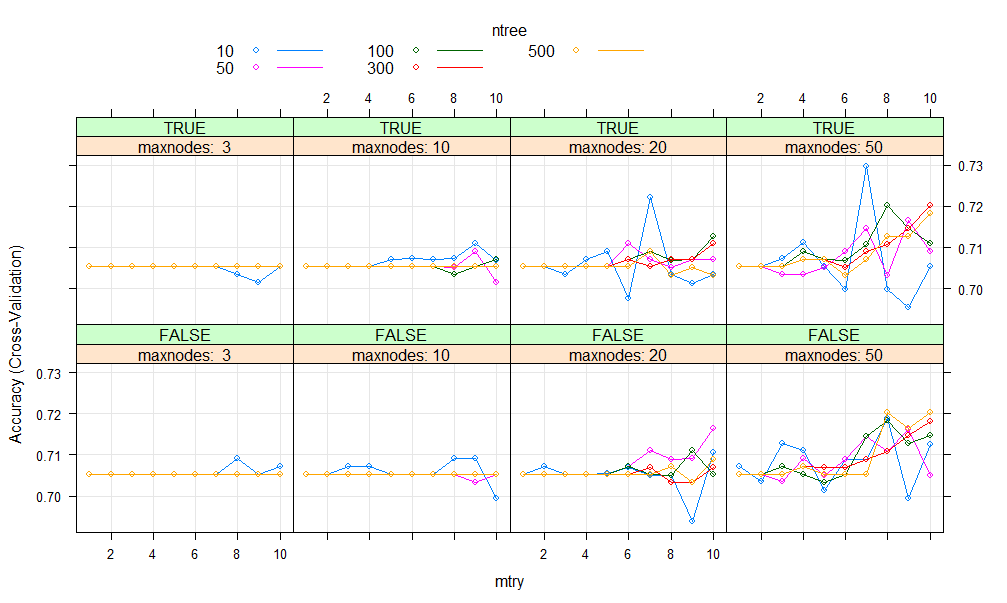
\includegraphics[scale=0.60]{tex/customD_vol4.png}
 \caption{Dokładność predykcji modelu dla klasy spożywającej alkohol w tygodniu w zależności od różnych kombinacji parametrów.}
 \label{fig:classes}
\end{figure}

    % #mtry ntree maxnodes replace
% #248    7    10       50    TRUE

Na podstawie przeprowadzonych badań dla spożywania alkoholu w tygodniu okazuje się model zbudowany z 10 drzew oraz 7 atrybutów wykorzystywanych do  budowania podziału, maksymalnie 50 węzłów w drzewie oraz wykorzystywania losowania ze zwracaniem.


 OOB estimate of  error rate: 29.62\%
 

 Confusion matrix:
 
   1  2 3 4 5   class.error
   
 1 343 14 5 0 2  0.05769231
 
 2  68 19 6 0 0  0.79569892
 
 3  22 10 3 0 2  0.91891892
 
 4   5  3 2 0 2  1.00000000
 
 
 5  10  0 3 0 1  0.92857143
\begin{table}[h]
\begin{tabular}{|c|c|c|c|c|c|c|}
\hline
\multirow{}{}{\textbf{X (Wartość prawdziwa)}} & \multicolumn{5}{c|}{\textbf{Y (Predykcja)}}                                & \multirow{}{}{\textbf{błąd klasy}} \\ \cline{2-6}
                            & \textbf{1} & \textbf{2} & \textbf{3} & \textbf{4} & \textbf{5} &                                      \\ \hline
\textbf{1}                  & 343        & 14         & 5          & 0          & 2          & 0.05769231                           \\ \hline
\textbf{2}                  & 68         & 19         & 6          & 0          & 0          & 0.79569892                           \\ \hline
\textbf{3}                  & 22         & 10         & 3          & 0          & 2          & 0.91891892                           \\ \hline
\textbf{4}                  & 5          & 3          & 2          & 0          & 1          & 1.0000000                            \\ \hline
\textbf{5}                  & 10         & 0          & 3          & 0          & 1          & 0.92857143                           \\ \hline
\end{tabular}
\end{table}

Łączna wartość błędu out-of-bag to 29.62\%, co oznacza że dokładnie 70.38\% próbek zostało poprawnie sklasyfikowanych. 

\begin{figure}[h]
     \centering 
     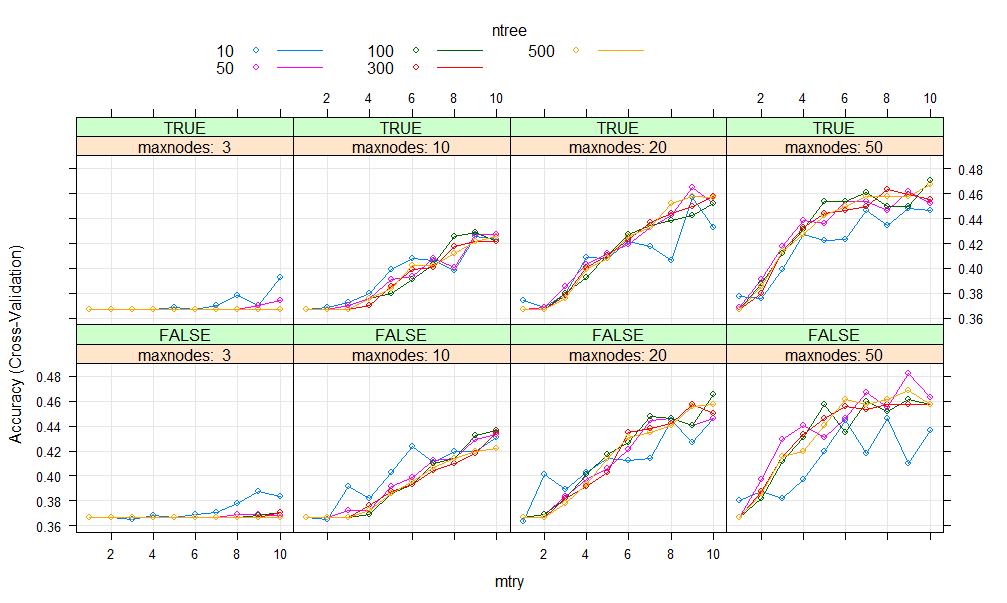
\includegraphics[scale=0.60]{tex/customW_vol4.png}
     \caption{Dokładność predykcji modelu dla klasy spożywającej alkohol w weekend w zależności od różnych kombinacji parametrów.}
     \label{fig:classes}
\end{figure}


% plot(custom_W)
% #     mtry ntree maxnodes replace
% # 335    9    50       50   FALSE

Na podstawie przeprowadzonych badań dla spożywania alkoholu w weekend okazuje się model zbudowany z 50 drzew oraz 9 atrybutów wykorzystywanych do  budowania podziału oraz maksymalnie 50 węzłów w drzewie oraz niewykorzystywania losowania ze zwracaniem.
% tabela
 OOB estimate of  error rate: 55.77\%
 
Confusion matrix:

   1  2  3  4 5 class.error
   
 1 179  7  7  0 1  0.07731959
 
 2  88 13 15  7 0  0.89430894
 
 3  50 18 12 22 1  0.88349515
 
 4  25  9 21 22 1  0.71794872
 
 5   7  3  5  8 8  0.74193548
 \begin{table}[h!]
\begin{tabular}{|c|c|c|c|c|c|c|}
\hline
\multirow{}{}{\textbf{Wartość  prawdziwa}} & \multicolumn{5}{c|}{\textbf{ Predykcja}}                                & \multirow{}{}{\textbf{błąd klasy}} \\ \cline{2-6}
                            & \textbf{1} & \textbf{2} & \textbf{3} & \textbf{4} & \textbf{5} &                                      \\ \hline
\textbf{1}                  & 179        & 7          & 7          & 0          & 1          & 0.07731959                           \\ \hline
\textbf{2}                  & 88         & 13         & 15         & 7          & 0          & 0.894303984                          \\ \hline
\textbf{3}                  & 50         & 18         & 12         & 22         & 1          & 0.88439515                           \\ \hline
\textbf{4}                  & 25         & 9          & 21         & 22         & 1          & 0.71794872                           \\ \hline
\textbf{5}                  & 7          & 3          & 5          & 8          & 8          & 0.74193548                           \\ \hline
\end{tabular}
\end{table}
Łączna wartość błędu out-of-bag to 55.77\%, co oznacza że dokładnie 44.23\% próbek zostało poprawnie sklasyfikowanych. 

\todo{przepuścic to jeszcze bez ntree = 1 ? żeby wykres byl bardziej czytelny??.}


Podsumowując, 

% -waga klas (classwt)
% -losowanie ze zwracaniem (replace)


\todo{jeszcze wagi to do .}

